% This file was created by matlab2tikz.
%
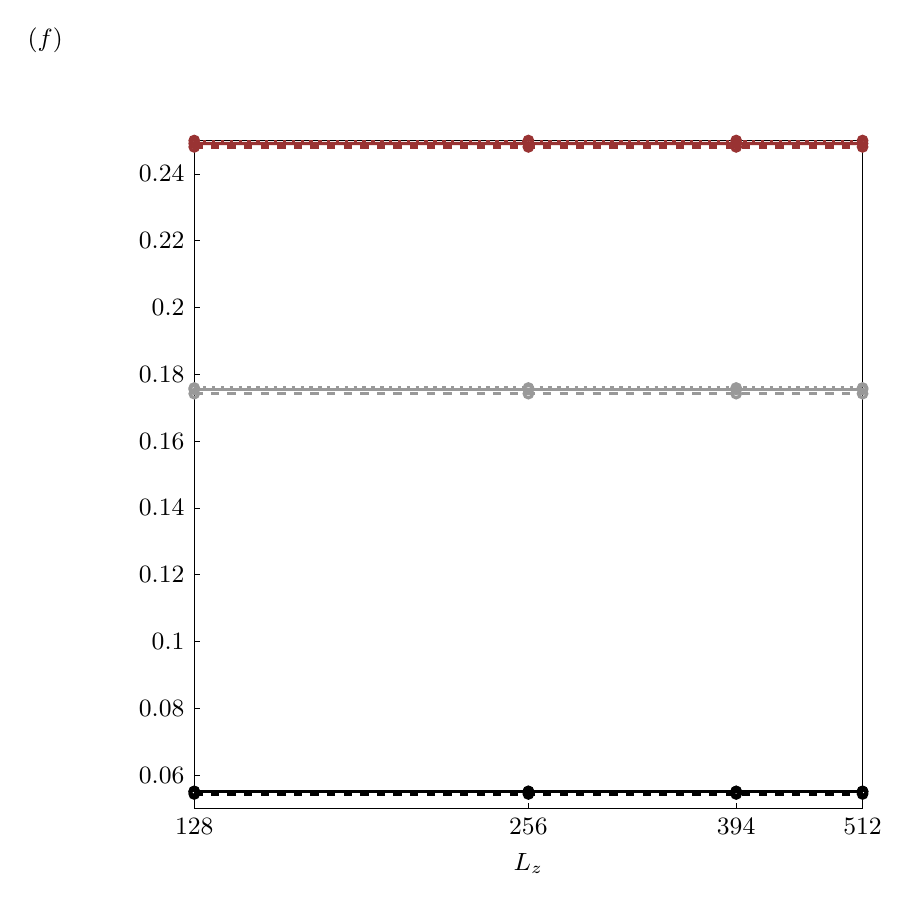
\begin{tikzpicture}

\begin{axis}[%
width=11.255in,
height=7.131in,
at={(1.888in,0.962in)},
scale only axis,
clip=true,
separate axis lines,
every outer x axis line/.append style={black},
every x tick label/.append style={font=\color{black}},
every x tick/.append style={black},
xmode=log,
xmin=128,
xmax=512,
xtick={128,256,394,512},
xticklabels={{128},{256},{394},{512}},
xminorticks=true,
xlabel={$L_z$},
every outer y axis line/.append style={black},
every y tick label/.append style={font=\color{black}},
every y tick/.append style={black},
ymin=0.05,
ymax=0.25,
axis background/.style={fill=white},
clip=true,
clip mode=individual,
axis lines=box,
xtick pos=bottom,
ytick pos=left,
tick align=inside,
major tick length=2pt,
width=0.7\linewidth,
height=0.7\linewidth,
every axis/.append style={font=\fontsize{9}{9}\selectfont},xlabel style={font=\fontsize{9}{9}\selectfont},title style={font=\fontsize{9}{9}\selectfont},
legend style={font=\fontsize{8}{9}\selectfont,inner sep=1pt,row sep=1pt,column sep=2pt,nodes={scale=1.00},draw=none},legend image post style={xscale=0.35},
legend columns=1,
scaled x ticks=false,
tick label style={/pgf/number format/fixed,/pgf/number format/precision=2},
every x tick label/.append style={font=\fontsize{9}{9}\selectfont\color{black}},
every y tick label/.append style={font=\fontsize{9}{9}\selectfont\color{black}},
,,
colormap={sigmamap}{rgb(0.0000)=(0.0200,0.1880,0.3800); rgb(0.1000)=(0.0743,0.3456,0.5616); rgb(0.2000)=(0.1918,0.4980,0.7060); rgb(0.3000)=(0.3890,0.6708,0.8226); rgb(0.4000)=(0.7552,0.8682,0.9228); rgb(0.5000)=(0.9690,0.9689,0.9689); rgb(0.6000)=(0.9425,0.8044,0.7614); rgb(0.7000)=(0.8767,0.4910,0.4020); rgb(0.8000)=(0.7869,0.2866,0.2470); rgb(0.9000)=(0.6186,0.1239,0.1568); rgb(1.0000)=(0.4040,0.0000,0.1220)}
]
\addplot [color=black, line width=1.2pt, mark size=1.5pt, mark=o, mark options={solid, black}, forget plot]
  table[row sep=crcr]{%
128	0.0551657662861021\\
256	0.0551657671452841\\
394	0.0551657670740398\\
512	0.0551657662787053\\
};
\addplot [color=black, dashed, line width=1.2pt, mark size=1.5pt, mark=o, mark options={solid, black}, forget plot]
  table[row sep=crcr]{%
128	0.0544082204400931\\
256	0.0544082214671291\\
394	0.0544082219107181\\
512	0.0544082211526974\\
};
\addplot [color=black, dotted, line width=1.2pt, mark size=1.5pt, mark=o, mark options={solid, black}, forget plot]
  table[row sep=crcr]{%
128	0.0551352319432771\\
256	0.055135231204971\\
394	0.0551352322341404\\
512	0.0551352314177145\\
};
\addplot [color=white!60!black, line width=1.2pt, mark size=1.5pt, mark=o, mark options={solid, white!60!black}, forget plot]
  table[row sep=crcr]{%
128	0.175471928143913\\
256	0.175471928839631\\
394	0.175471928614474\\
512	0.17547192819531\\
};
\addplot [color=white!60!black, dashed, line width=1.2pt, mark size=1.5pt, mark=o, mark options={solid, white!60!black}, forget plot]
  table[row sep=crcr]{%
128	0.174205451609595\\
256	0.174205451477413\\
394	0.174205451144942\\
512	0.174205450486856\\
};
\addplot [color=white!60!black, dotted, line width=1.2pt, mark size=1.5pt, mark=o, mark options={solid, white!60!black}, forget plot]
  table[row sep=crcr]{%
128	0.175893008924764\\
256	0.17589300936865\\
394	0.175893008672956\\
512	0.175893008327821\\
};
\addplot [color=red!60!teal, line width=1.2pt, mark size=1.5pt, mark=o, mark options={solid, red!60!teal}, forget plot]
  table[row sep=crcr]{%
128	0.249057456773047\\
256	0.249057456595799\\
394	0.249057457261426\\
512	0.2490574589601\\
};
\addplot [color=red!60!teal, dashed, line width=1.2pt, mark size=1.5pt, mark=o, mark options={solid, red!60!teal}, forget plot]
  table[row sep=crcr]{%
128	0.248046962665486\\
256	0.248046962579005\\
394	0.248046962400925\\
512	0.248046960927033\\
};
\addplot [color=red!60!teal, dotted, line width=1.2pt, mark size=1.5pt, mark=o, mark options={solid, red!60!teal}, forget plot]
  table[row sep=crcr]{%
128	0.24994606976581\\
256	0.2499460699019\\
394	0.249946070292958\\
512	0.249946069178953\\
};
\node[right, align=left, inner sep=0]
at (rel axis cs:-0.25,1.15) {$(f)$};
\end{axis}
\end{tikzpicture}%